%!TEX program = xelatex

\documentclass[compress]{beamer}
%--------------------------------------------------------------------------
% Common packages
%--------------------------------------------------------------------------
\usepackage[english]{babel}
\usepackage{pgfpages} % required for notes on second screen
\usepackage{graphicx}
\usepackage{subfigure}
\usepackage{multicol}
\usepackage{multirow}
\def\block(#1,#2)#3{\multicolumn{#2}{c}{\multirow{#1}{*}{$ #3 $}}}

\usepackage{fontspec}

\usepackage{tabularx,ragged2e}
\usepackage{booktabs}

\usepackage{setspace}

\usepackage{gitdags}
\usepackage[normalem]{ulem} % strikeout
%--------------------------------------------------------------------------
% Load theme
%--------------------------------------------------------------------------
\usetheme{hri}

\usepackage{dtklogos} % must be loaded after theme
\usepackage{tikz}
\usetikzlibrary{intersections,arrows,shapes,calc,mindmap,backgrounds,positioning,svg.path}

\graphicspath{{figs/}}

\usepackage[cache]{minted}
\renewcommand{\theFancyVerbLine}{
  \sffamily\textcolor[rgb]{0.5,0.5,0.5}{\scriptsize\arabic{FancyVerbLine}}}

\newminted{java}{frame=lines,
                 linenos=true,
                 fontsize=\small,
                 xleftmargin=1.8em}

\newmintinline[java]{java}{fontsize=\small}

\newminted{sh}{frame=lines,
                 linenos=false,
                 fontsize=\small,
                 xleftmargin=1.8em}

\newmintinline[sh]{sh}{fontsize=\small}

\setbeamercolor{highlightCol}{bg=hriSec3,fg=white}
\newcommand{\highlight}[1]{%
    \vspace{1em}%
    \begin{beamercolorbox}[wd=\linewidth,ht=2ex,dp=0.7ex]{highlightCol}%
    \centering #1%
    \end{beamercolorbox}%
    \vspace{1em}%
}%

\tikzset{temporal/.code args={<#1>#2#3#4}{%
          \temporal<#1>{\pgfkeysalso{#2}}{\pgfkeysalso{#3}}{\pgfkeysalso{#4}} % \pgfkeysalso doesn't change the path
}}


%--------------------------------------------------------------------------
% General presentation settings
%--------------------------------------------------------------------------
\title{\Medium git}
\subtitle{the basics}
\date{12 Feb. 2016}
\author{Séverin Lemaignan}
\institute{Centre for Robotics \& Neural
Systems\\{\Medium Plymouth University}}

%--------------------------------------------------------------------------
% Notes settings
%--------------------------------------------------------------------------
%\setbeameroption{show notes on second screen}
%\setbeameroption{hide notes}

\begin{document}

\maketitle

%%%%%%%%%%%%%%%%%%%%%%%%%%%%%%%%%%%%%%%%%%%%%%%%%%%%%%%%%%%%%%%%%%%%%%%%%%%%%%%

\imageframe{}{zipfiles.pdf}
\imageframe{}{dropbox_zipfiles.pdf}

{
    \fullbackground{../figs/facebook-wall.png}
    \begin{frame}[plain]{}
        \only<2>{
            \begin{center}
                
\includegraphics[width=\linewidth]{devil}
            \end{center}
        }
    \end{frame}
}

\section{Code versioning}

\begin{frame}{Why code versioning?}

    \begin{itemize}
        \item The history of your development
        \item Compare the current code with an older version
        \item Roll-back to previous versions
        \item Experiment without losing anything
        \item Trace who did what (at the level of the line of code)
        \item Annotate your workflow (important milestones, etc)
        \item Avoid catastrophes!
    \end{itemize}
\end{frame}

\begin{frame}{Atomic commits}

    The single most important concept (because it requires to think about
    development in terms of {\Medium functional units}):

    \highlight{Atomic commit}

    \only<1>{
        A (typically small) commit that represent a {\Medium single, coherent \&
    complete} functional change.
    }
    \only<2>{
    \begin{itemize}
        \item Easy to understand the change
        \item Debugging made easy (\texttt{git bisect})
        \item Collaboration made easy (less, smaller conflict)
        \item Easy to write a useful commit message
    \end{itemize}
    }

\end{frame}

\begin{frame}[fragile]{}

\centering

\begin{tikzpicture}[
    >=latex,
    every edge/.style={draw,thick,hriSec3},
    file/.style={align=left, inner sep=1pt,font=\scriptsize\tt}
]

\node at (-2, 1.5)[file,temporal=<4>{red}{black}{white}] (file1) {\sout{main.cpp}};
\node [file,temporal=<4>{red}{black}{white},below=0.0 of file1.south east,anchor=north east] (file2) {src/main.cpp};
\node [file,temporal=<2>{red}{black}{white},below=0.0 of file2.south east, anchor=north east] (file3) {src/position.cpp};
\node [file,temporal=<2>{red}{black}{white},below=0.0 of file3.south east,anchor=north east] (file4) {src/position.hpp};
\node [file,temporal=<3>{red}{black}{white},below=0.0 of file4.south east,anchor=north east] (file5) {share/model.csv};


    \onslide<2>{
        \gitDAG[grow right sep = 2em]{
            A;
        };

        \gitbranch
        {master}
        {above=of A}
        {A}

        \gitHEAD
        {above=of master}
        {master}


    \path[draw] (file3.east) edge [->, bend left] (A);
    \path[draw] (file4.east) edge [->, bend left] (A);

    }
    \onslide<3>{
        \gitDAG[grow right sep = 2em]{
            A -- B;
        };

        \gitbranch
        {master}
        {above=of B}
        {B}

        \gitHEAD
        {above=of master}
        {master}

        \path[draw] (file5.east) edge [->, bend left,hriSec2] (B);
    }

    \onslide<4->{
        \gitDAG[grow right sep = 2em]{
            A -- B -- C;
        };

        \gitbranch
        {master}     % node name and text 
        {above=of C} % node placement
        {C}          % target

        \gitHEAD
        {above=of master} % node placement
        {master}          % target

        \path[draw] (file1.east) edge [->, bend left,hriSec1Comp] (C);
        \path[draw] (file2.east) edge [->, bend left,hriSec1Comp] (C);
    }

\end{tikzpicture}

\vspace{3em}
\small
\only<2>{
\texttt{git add src/position.*}\\
\texttt{git commit -m"Fix computation of position (float->double)"}
}
\only<3>{
\texttt{git add share/model.csv}\\
\texttt{git commit -m"Re-trained model with 52 more participants"}
}
\uncover<4>{
\texttt{git add src/main.*}\\
\texttt{git commit -m"Move main.cpp to src/"}
}

\end{frame}

\begin{frame}[fragile]{Log}
\begin{shcode}
$ git log
commit fa009cd7fca05b0b61170b20cf76a5f72b8843c2
Author: Severin Lemaignan <severin.lemaignan@plymouth.ac.uk>
Date:   Wed Feb 10 16:48:22 2016 +0000

    Move main.cpp to src/

commit aff81119459d9193c09effef1c150c4f7eac08dc
Author: Severin Lemaignan <severin.lemaignan@plymouth.ac.uk>
Date:   Wed Feb 10 16:48:02 2016 +0000

    Re-trained model with 52 more participants

commit 4113b9b6e6bbc8de532ad90153e0059cb5819de7
Author: Severin Lemaignan <severin.lemaignan@plymouth.ac.uk>
Date:   Wed Feb 10 16:47:46 2016 +0000

    Fix computation of position (float->double)
\end{shcode}


\end{frame}

\begin{frame}{}

\centering

\begin{tikzpicture}
        \gitDAG[grow right sep = 2em]{
            4113b9 -- aff811 -- fa009c;
        };

        \gitbranch
        {master}     % node name and text 
        {above=of fa009c} % node placement
        {fa009c}          % target

        \gitHEAD
        {above=of master} % node placement
        {master}          % target

\end{tikzpicture}

\end{frame}

\begin{frame}{The staging area}
    \centering
    \only<1>{
        But why do we have to manually tell Git what files to add or remove?
    }
    \only<2>{
        No ``commit all changes'' by default {\tiny (well, you
        can, actually...)}\\
        $\Rightarrow$ Help thinking in terms of atomic commits!
    }
    \only<3->{
        Preparing a commit consists in filling the {\Medium staging area} (or
        {\Medium index}) with the list of changes:

        \begin{tikzpicture}[
                >=latex,
                every edge/.style={draw,thick,hriSec3},
                file/.style={align=left, inner sep=1pt,font=\scriptsize\tt}
            ]

            \node at (-3.5, 2)[file,red] (file1) {\sout{main.cpp}};
            \node [file,red,below=0.0 of file1.south east,anchor=north east] (file2) {src/main.cpp};
            \node [file,temporal=<3>{red}{black}{white},below=0.0 of file2.south east, anchor=north east] (file3) {src/position.cpp};
            \node [file,temporal=<3>{red}{black}{white},below=0.0 of file3.south east,anchor=north east] (file4) {src/position.hpp};
            \node [file,red,below=0.0 of file4.south east,anchor=north east] (file5) {share/model.csv};


            \node[gitSA,] (stagingarea) at (-2.5,3) {staging area};

            \onslide<3>{
                \gitDAG[grow right sep = 2em]{
                    154ce2 -- f327ba;
                };

                \gitbranch
                {master}     % node name and text 
                {above=of f327ba} % node placement
                {f327ba}          % target

                \gitHEAD
                {above=of master} % node placement
                {master}          % target



                \path[draw] (file3.east) edge [->, bend right,hriSec1Comp] (stagingarea);
                \path[draw] (file4.east) edge [->, bend right,hriSec1Comp] (stagingarea);

            }
            \onslide<4>{
                \gitDAG[grow right sep = 2em]{
                    154ce2 -- f327ba -- 4113b9;
                };

                \gitbranch
                {master}     % node name and text 
                {above=of 4113b9} % node placement
                {4113b9}          % target

                \gitHEAD
                {above=of master} % node placement
                {master}          % target

                \node[highlighted commit] at (4113b9) {\phantom{4113b9}};
                \draw[resetarrows] ([xshift=-1em,yshift=-1em]stagingarea.east) to[bend
                left] (4113b9.north west);

            }



        \end{tikzpicture}


        \only<3>{
            \texttt{git add}\\
            \texttt{git rm}\\
            \texttt{git add -p}\\
            ...\\
        }
        \only<4>{
            ~\\
            \texttt{git commit}\\
            ~\\
            ~\\
        }


    }
\end{frame}

\begin{frame}[fragile]{To summarize...}

The first time...
\begin{shcode}
$ mkdir my_repo && cd my_repo
$ git init
\end{shcode}
Then...
\begin{shcode}
# make some changes...
$ git add <files>
$ git commit -m"<commit message>"
# make some changes...
$ git add <files>
$ git commit -m"<other commit message>"
# That's it!
\end{shcode}


\end{frame}


\begin{frame}{}
    \centering
    Viewed from a GUI\\
    {\Medium GitHub for Windows} (GHfW) Walkthrough\par
    \vspace{3em}
    \url{https://desktop.github.com/}
\end{frame}

\imageframe[black]{Log in to your GitHub account}{github-windows/1}
\imageframe[black]{Create a (local) repository}{github-windows/2}
\imageframe[black]{GHfW has already made a first commit on your behalf}{github-windows/3}
\imageframe[black]{Open the repo in Windows Explorer}{github-windows/4}
\imageframe[black]{Add a simple \texttt{README.md}...}{github-windows/5}
\imageframe[black]{Back to GHfW: the change is listed in the {\Medium Changes} panel}{github-windows/6}
\imageframe[black]{Write a commit message \& commit!}{github-windows/7}
\imageframe[black]{The {\Medium History} panel shows the log and a diff of your changes}{github-windows/8}

\begin{frame}{Branches}

    \centering

    \begin{tikzpicture}
        \only<1-5>{
        \onslide<1>{
            \gitDAG[grow right sep = 2em]{
                A -- B -- C;
            };

            % Branch
            \gitbranch
            {master}     % node name and text 
            {above=of C} % node placement
            {C}          % target

            % HEAD reference
            \gitHEAD
            {above=of master} % node placement
            {master}          % target

        }

        \onslide<2>{
            \gitDAG[grow right sep = 2em]{
                A -- B -- C;
            };

            % Branch
            \gitbranch
            {master}     % node name and text 
            {above=of C} % node placement
            {C}          % target

            \gitbranch
            {cool-idea}     % node name and text 
            {above=of master} % node placement
            {master}          % target

            % HEAD reference
            \gitHEAD
            {above=of cool-idea} % node placement
            {cool-idea}          % target
        }

        \onslide<3>{
            \gitDAG[grow right sep = 2em]{
                A -- B -- C -- D -- E;
            };

            % Branch
            \gitbranch
            {master}     % node name and text 
            {above=of C} % node placement
            {C}          % target

            \gitbranch
            {cool-idea}     % node name and text 
            {above=of E} % node placement
            {E}          % target

            % HEAD reference
            \gitHEAD
            {above=of cool-idea} % node placement
            {cool-idea}          % target
        }

        \onslide<4>{
            \gitDAG[grow right sep = 2em]{
                A -- B -- C -- D -- E;
            };

            % Branch
            \gitbranch
            {master}     % node name and text 
            {above=of C} % node placement
            {C}          % target

            \gitbranch
            {cool-idea}     % node name and text 
            {above=of E} % node placement
            {E}          % target

            % HEAD reference
            \gitHEAD
            {above=of master} % node placement
            {master}          % target
        }

        \onslide<5>{
            \gitDAG[grow right sep = 2em]{
                A -- B -- C -- {
                    D -- E,
                    F -- G -- H,
                }
            };

            % Branch
            \gitbranch
            {master}     % node name and text 
            {above=of H} % node placement
            {H}          % target

            \gitbranch
            {cool-idea}     % node name and text 
            {above=of E} % node placement
            {E}          % target

            % HEAD reference
            \gitHEAD
            {above=of master} % node placement
            {master}          % target
        }
    }
        \only<6->{
            \gitDAG[grow right sep = 1.5em]{
                A -- B -- C -- {
                    D -- E,
                    F -- G -- H -- {
                        K,
                        I -- J
                        },
                }
            };

            % Branch
            \gitbranch
            {master}     % node name and text 
            {above=of K} % node placement
            {K}          % target

            \gitbranch
            {cool-idea}     % node name and text 
            {above=of E} % node placement
            {E}          % target

            \gitbranch
            {bug142}     % node name and text 
            {above=of J} % node placement
            {J}          % target


            % HEAD reference
            \gitHEAD
            {above=of master} % node placement
            {master}          % target
        }


    \end{tikzpicture}

    \vspace{3em}
    \centering
    \only<1>{
        What if...?\\
    }
    \only<2>{
        \Large
        \texttt{git checkout -b cool-idea}\\
    }
    \only<5>{
        The branch name is an alias for the tip of the current branch\\
    }
    \only<6>{
        $\Rightarrow$ branches are very cheap\\ 
        +10 of them at a given time it not uncommon\\
    }
    \uncover<4>{
        Let go back to serious stuff!\\
        \Large
        \texttt{git checkout master}
    }


\end{frame}


\begin{frame}{Merging branches}

    \centering

\begin{tikzpicture}[
    >=latex,
    every edge/.style={draw,thick,hriSec3}
]

        \onslide<1>{
            \gitDAG[grow right sep = 2em]{
                B -- C -- {
                    D -- E,
                    F -- G -- H,
                };
            };

            % Branch
            \gitbranch
            {master}     % node name and text 
            {above=of H} % node placement
            {H}          % target

            \gitbranch
            {cool-idea}     % node name and text 
            {above=of E} % node placement
            {E}          % target

            % HEAD reference
            \gitHEAD
            {above=of master} % node placement
            {master}          % target

            \node[DAGcommit,right=3 of E.south,dashed] (merge) {?};
            \path[draw] (E) edge [->, bend left] (merge);
            \path[draw] (H) edge [->, bend right] (merge);
    }
        \onslide<2>{
            \gitDAG[grow right sep = 2em]{
                B -- C -- {
                    D -- E,
                    F -- G -- H -- merge,
                };

                E -- merge;
            };

            % Branch
            \gitbranch
            {master}     % node name and text 
            {above=of merge} % node placement
            {merge}          % target

            \gitbranch
            {cool-idea}     % node name and text 
            {above=of E} % node placement
            {E}          % target

            % HEAD reference
            \gitHEAD
            {above=of master} % node placement
            {master}          % target

    }
        \onslide<3>{
            \gitDAG[grow right sep = 2em]{
                B -- C -- {
                    D -- E,
                    F -- G -- H -- I -- J,
                };

                E -- I;
            };

            % Branch
            \gitbranch
            {master}     % node name and text 
            {above=of J} % node placement
            {J}          % target

            \gitbranch
            {cool-idea}     % node name and text 
            {above=of E} % node placement
            {E}          % target

            % HEAD reference
            \gitHEAD
            {above=of master} % node placement
            {master}          % target

    }
        \onslide<4>{
            \gitDAG[grow right sep = 2em]{
                B -- C -- {
                    D -- E -- K -- L,
                    F -- G -- H -- I -- J,
                };

                E -- I;
            };

            % Branch
            \gitbranch
            {master}     % node name and text 
            {above=of J} % node placement
            {J}          % target

            \gitbranch
            {cool-idea}     % node name and text 
            {above=of L} % node placement
            {L}          % target

            % HEAD reference
            \gitHEAD
            {above=of cool-idea} % node placement
            {cool-idea}          % target

    }



    \end{tikzpicture}

    \vspace{3em}
    \centering
    \only<1>{
        Two options: {\Medium merging} and {\Medium rebasing}\\
    }
    \only<2>{
        Merging\\
        \Large
        \texttt{git merge cool-idea}\\
    }
    \only<3>{
        \Large
        \texttt{git commit}\\
    }
    \uncover<4>{
        \Large
        \texttt{git checkout cool-idea}\\
        \texttt{git commit}\\
        \normalsize
        ...etc.
    }


\end{frame}

\begin{frame}{Rebasing branches}

    \centering

\begin{tikzpicture}[
    >=latex,
    every edge/.style={draw,thick,hriSec3}
]

        \onslide<1>{
            \gitDAG[grow right sep = 2em]{
                B -- C -- {
                    D -- E,
                    F -- G -- H,
                };
            };

            % Branch
            \gitbranch
            {master}     % node name and text 
            {above=of H} % node placement
            {H}          % target

            \gitbranch
            {cool-idea}     % node name and text 
            {above=of E} % node placement
            {E}          % target

            % HEAD reference
            \gitHEAD
            {above=of master} % node placement
            {master}          % target

            \node[DAGcommit,right=3 of E.south,dashed] (merge) {?};
            \path[draw] (E) edge [->, bend left] (merge);
            \path[draw] (H) edge [->, bend right] (merge);
    }
        \onslide<2>{
            \gitDAG[grow right sep = 2em]{
                B -- C -- {
                    D -- E -- F' -- G' -- H',
                    {[nodes=unreachable] F -- G -- H },
                };
            };

            % Branch
            \gitbranch
            {master}     % node name and text 
            {above=of H'} % node placement
            {H'}          % target

            \gitbranch
            {cool-idea}     % node name and text 
            {above=of E} % node placement
            {E}          % target

            % HEAD reference
            \gitHEAD
            {above=of master} % node placement
            {master}          % target

    }
        \onslide<3>{
            \gitDAG[grow right sep = 2em]{
                B -- C -- {
                    D -- E -- {
                        I -- J,
                        F' -- G' -- H',
                    },
                    {[nodes=unreachable] F -- G -- H },
                };
            };

            % Branch
            \gitbranch
            {master}     % node name and text 
            {above=of H'} % node placement
            {H'}          % target

            \gitbranch
            {cool-idea}     % node name and text 
            {above=of J} % node placement
            {J}          % target

            % HEAD reference
            \gitHEAD
            {above=of cool-idea} % node placement
            {cool-idea}          % target

    }

    \end{tikzpicture}

    \vspace{3em}
    \centering
    \only<2>{
        Rebasing\\
        \Large
        \texttt{git rebase cool-idea}\\
    }
    \uncover<3>{
        \Large
        \texttt{git checkout cool-idea}\\
        \texttt{git commit}\\
    }


\end{frame}

\begin{frame}{More commit aliases: Tags}

    \centering

    \begin{tikzpicture}
            \gitDAG[grow right sep = 1.5em]{
                A -- B -- C -- {
                    D -- E,
                    F -- G -- H -- {
                        K,
                        I -- J
                        },
                }
            };

            \gittag
            [v12]
            {v1.2}
            {above=of C}
            {C}

            \gitbranch
            {master}
            {above=of K}
            {K}

            \gitbranch
            {cool-idea}
            {above=of E}
            {E}

            \gitbranch
            {bug142}
            {above=of J}
            {J}

            \gittag
            {WP5}
            {above=of H}
            {H}


            % HEAD reference
            \gitHEAD
            {above=of master} % node placement
            {master}          % target


    \end{tikzpicture}

    \vspace{3em}
    \centering
        {\Medium Label} important commits/milestones\\
        \Large
        \texttt{git tag v1.2}\\
        \texttt{git tag WP5}


\end{frame}



\begin{frame}[fragile]{To summarize...}

\begin{shcode}
# where are we?
$ git branch
master
# make some changes...
$ git add <files> && git commit -m"<commit message>"
# start working on something new?
$ git checkout -b new-idea
$ git branch
new-idea
# work in that branch for a while
$ git add <files> && git commit -m"<commit message>"
# back to master
$ git checkout master
#...
# rebase master on new-idea: new-idea is now in master
$ git rebase new-idea
\end{shcode}

\end{frame}

\begin{frame}{}
    \centering
    {Viewed from a GUI...}
\end{frame}

\imageframe[black]{We can easily create a new branch}{github-windows/9}
\imageframe[black]{We can compare \texttt{numerical\_coordinates} with \texttt{master}\\ (click on {\Medium View branch} for the full history)}{github-windows/10}
\imageframe[black]{We can jump between branches...}{github-windows/11}
\imageframe[black]{...and watch how they diverge}{github-windows/12}
\imageframe[black]{We switch back to \texttt{numerical\_coordinates} and merge in \texttt{master}}{github-windows/13}
\imageframe[black]{The merge commit is reflected in the history of the branch}{github-windows/14}

\section{Collaborating}

\imageframe{}{dvcs-1}
\imageframe{}{dvcs-2}
\imageframe{}{dvcs-3}
\imageframe{}{dvcs-4}
\imageframe{}{dvcs-5}
\imageframe{}{dvcs-6}
\imageframe{}{dvcs-7}
\imageframe{}{dvcs-8}



\begin{frame}[fragile]{}

\centering

    \begin{tikzpicture}
    % Commit DAG
    \onslide<1-3>{
      \gitDAG[grow right sep = 2em]{
        A -- B -- C;
      };

      % Branch
      \gitbranch
        {master}     % node name and text 
        {above=of C} % node placement
        {C}          % target
    }



      % HEAD reference
    \onslide<1-2>{
      \gitHEAD
        {above=of master} % node placement
        {master}          % target
    }

    \onslide<3>{
      \gitremotebranch
        [origmaster]    % node name
        {origin/master} % node text
        {above=of master}    % node placement
        {master}             % target
      \gitHEAD
        {above=of origmaster} % node placement
        {origmaster}          % target
    }

    \end{tikzpicture}

\vspace{3em}
    \begin{overlayarea}{\textwidth}{5cm}
\only<2>{
\small
\texttt{git remote add origin git@github.com:user/repo.git}\par
\scriptsize
\texttt{git remote add john-usb E:\textbackslash john\_repo}\\
\texttt{git remote add ftp-origin ftp://host.xz/path/to/repo.git/}\\
...\\
}

\only<3>{
\Large
\texttt{git push origin master} \par
\normalsize
(or simply \texttt{git push})
}
\end{overlayarea}
\end{frame}

\begin{frame}[fragile]{}

    \centering

    \begin{tikzpicture}
        \onslide<1-2>{
            \gitDAG[grow right sep = 2em]{
                A -- B -- C -- D -- E;
            };

            % Branch
            \gitbranch
            {master}     % node name and text 
            {above=of E} % node placement
            {E}          % target

            % HEAD reference
            \gitHEAD
            {above=of master} % node placement
            {master}          % target

            \gitremotebranch
            [origmaster]    % node name
            {origin/master} % node text
            {above=of C}    % node placement
            {C}             % target
        }

        \onslide<3>{
            \gitDAG[grow right sep = 2em]{
                A -- B -- C -- {
                    F,
                    D -- E,
                }
            };

            % Branch
            \gitbranch
            {master}     % node name and text 
            {above=of E} % node placement
            {E}          % target

            % HEAD reference
            \gitHEAD
            {above=of master} % node placement
            {master}          % target

            \gitremotebranch
            [origmaster]    % node name
            {origin/master} % node text
            {above=of F}    % node placement
            {F}             % target
        }

        \onslide<4-5>{
            \gitDAG[grow right sep = 2em]{
                A -- B -- C -- {
                    F -- D' -- E',
                    {[nodes=unreachable] D -- E },
                }
            };

            % Branch
            \gitbranch
            {master}     % node name and text 
            {above=of E'} % node placement
            {E'}          % target

            % HEAD reference
            \gitHEAD
            {above=of master} % node placement
            {master}          % target

            \gitremotebranch
            [origmaster]    % node name
            {origin/master} % node text
            {above=of F}    % node placement
            {F}             % target
        }

        \onslide<6->{
            \gitDAG[grow right sep = 2em]{
                A -- B -- C -- {
                    F -- D' -- E',
                    {[nodes=unreachable] D -- E },
                }
            };

            % Branch
            \gitbranch
            {master}     % node name and text 
            {above=of E'} % node placement
            {E'}          % target


            \gitremotebranch
            [origmaster]    % node name
            {origin/master} % node text
            {above=of master}    % node placement
            {master}             % target

            \gitHEAD
            {above=of origmaster} % node placement
            {origmaster}          % target
        }


    \end{tikzpicture}

    \vspace{3em}
    \begin{overlayarea}{\textwidth}{5cm}
    \only<2>{
        What happened on our remote? Let's have a look...\\
        \Large
        \texttt{git fetch origin}\\
    }

    \only<4>{
        \Large
        \texttt{git rebase origin/master}\par
        \normalsize
        (but you don't need it, because...)\\
    }
    \only<5>{
        \Large
        \texttt{git pull --rebase}\\
    }
    \only<6>{
        \Large
        \texttt{git push}\\
    }
    \end{overlayarea}

\end{frame}



\begin{frame}[fragile]{To summarize...}

The first time...
\begin{shcode}
$ git clone <url>
# for instance,
# git clone https://github.com/user/repo.git
\end{shcode}
Then...
\begin{shcode}
$ cd <repo>
# make some changes...
$ git add <files>
$ git commit -m"<commit message>"
# ...
# when you want to share:
$ git pull --rebase # any changes on the remote?
$ git push
\end{shcode}

\end{frame}

\section{Social coding: GitHub workflow}

\imageframe[black]{\Medium GitHub}{github-morse}
\imageframe[black]{\Medium BitBucket}{bitbucket}
\imageframe[black]{{\Medium GitLab} -- open-source\\You can install it on your own server}{gitlab}

\imageframe[black]{}{github-morse}

\imageframe{}{github-workflow-1}
\imageframe{}{github-workflow-2}
\imageframe{}{github-workflow-3}
\imageframe{}{github-workflow-4}
\imageframe{}{github-workflow-5}
\imageframe{}{github-workflow-6}


\begin{frame}[fragile]{What happened exactly?}

    \vspace{1em}
    \centering

    \begin{multicols}{2}
        \resizebox{\columnwidth}{!}{%
    \begin{tikzpicture}
        \onslide<1>{
            \gitDAG[grow right sep = 2em]{
                A -- B -- C -- D -- E;
            };

            % Branch
            \gitbranch
            {master}     % node name and text 
            {above=of E} % node placement
            {E}          % target

            % HEAD reference
            \gitHEAD
            {above=of master} % node placement
            {master}          % target

            \gitremotebranch
            [origmaster]    % node name
            {origin/master} % node text
            {above=of C}    % node placement
            {C}             % target
        }

        \onslide<2>{
            \gitDAG[grow right sep = 2em]{
                A -- B -- C -- {
                    F,
                    D -- E,
                }
            };

            % Branch
            \gitbranch
            {master}     % node name and text 
            {above=of E} % node placement
            {E}          % target

            \gitremotebranch
            [johnmaster]    % node name
            {john/master} % node text
            {above=1.2 of F}    % node placement
            {F}             % target


            \gitremotebranch
            [origmaster]    % node name
            {origin/master} % node text
            {above=of C}    % node placement
            {C}             % target

            \gitHEAD
            {above=of master} % node placement
            {master}          % target

        }

        \onslide<3>{
            \gitDAG[grow right sep = 2em]{
                A -- B -- C -- {
                    F -- D' -- E',
                    {[nodes=unreachable] D -- E },
                }
            };

            % Branch
            \gitbranch
            {master}     % node name and text 
            {above=of E'} % node placement
            {E'}          % target

            \gitremotebranch
            [origmaster]    % node name
            {origin/master} % node text
            {above=of C}    % node placement
            {C}             % target

            \gitremotebranch
            [johnmaster]    % node name
            {john/master} % node text
            {above=1.2 of F}    % node placement
            {F}             % target


            \gitHEAD
            {above=of master} % node placement
            {master}          % target


        }
        \onslide<4>{
            \gitDAG[grow right sep = 2em]{
                A -- B -- C -- {
                    F -- D' -- E',
                    {[nodes=unreachable] D -- E },
                }
            };

            % Branch
            \gitbranch
            {master}     % node name and text 
            {above=of E'} % node placement
            {E'}          % target

            \gitremotebranch
            [origmaster]    % node name
            {origin/master} % node text
            {above=of master}    % node placement
            {master}             % target

            \gitremotebranch
            [johnmaster]    % node name
            {john/master} % node text
            {above=1.2 of F}    % node placement
            {F}             % target


            \gitHEAD
            {above=of origmaster} % node placement
            {origmaster}          % target


        }

    \end{tikzpicture}
    }

    \only<1>{
        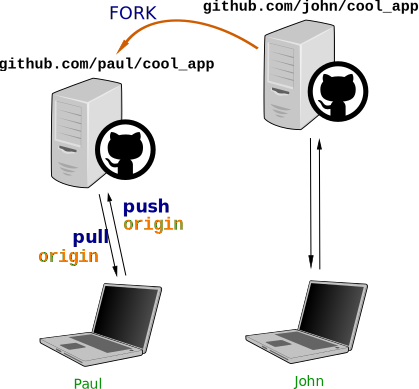
\includegraphics[width=0.8\columnwidth]{github-workflow-details-3}
    }
    \only<2-3>{
        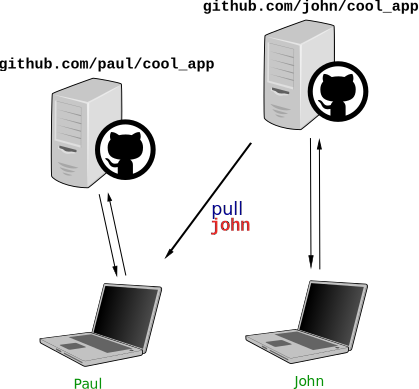
\includegraphics[width=0.8\columnwidth]{github-workflow-details-5}
    }

    \only<4>{
        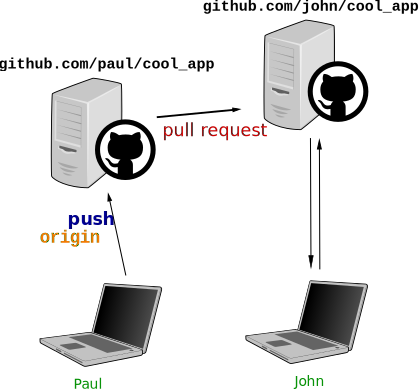
\includegraphics[width=0.8\columnwidth]{github-workflow-details-6}
    }

    \end{multicols}

    \begin{overlayarea}{\textwidth}{5cm}
    \only<1>{
        After forking on GitHub, Paul runs\\
        \texttt{git clone https://github.com/paul/cool\_app.git}\\
        \normalsize
        and he adds few local commits\\
    }

    \only<2>{
        He would like to propose his changes to John\\
        First, he needs to get the latest changes from John:\par
        \footnotesize
        \texttt{git add remote john https://github.com/john/cool\_app.git}\\
        \normalsize
        \texttt{git fetch john}\\
    }

    \only<3>{
        Paul rebases his \texttt{master} branch on John's one:\par
        \texttt{git rebase john/master}\par
        \footnotesize
        (actually, Paul would simply run \texttt{git pull --rebase john master})
    }
    \only<4>{
        He pushes his commits to his own GitHub account:\par
        \texttt{git push}\\
        ...and finally press the ``Create a pull request'' button in GitHub.
    }

\end{overlayarea}
\end{frame}

\begin{frame}{}
    \centering
    (what happens next on John's side is a story for another day :-) But to make
    it short, he can press ``Merge pull request'' on his GitHub account if he is
    happy with the pull-request!)
\end{frame}
\imageframe{}{github-workflow-7}


\section{The one slide to remember}

\begin{frame}{GIT cheat sheet}
\scriptsize
    \begin{multicols}{2}

    {\Medium To start...}\\
    ...from scratch: \texttt{git init}\\
    ...from existing repo: \texttt{git clone <url>}\par

    \rule{\columnwidth}{0.2pt}

    {\Medium Prepare commits:}\\
    \texttt{git add}\\
    \texttt{git rm}\\
    \texttt{git add -p} (partial files)\par

    {\Medium Commit:}\\
    \texttt{git commit}\par

    \rule{\columnwidth}{0.2pt}

    {\Medium Create branch:}\\
    \texttt{git checkout -b <branch>}\par

    {\Medium Jump between branches:}\\
    \texttt{git checkout <branch>}\par

    {\Medium ``Import'' another branch:}\\
    \texttt{git rebase <other\_branch>}\par

    \rule{\columnwidth}{0.2pt}

    {\Medium Add a remote source:}\\
    \texttt{git remote add <name> <url>}\par

    {\Medium What's new on a remote?}\\
    \texttt{git pull <remote> <branch>}\\
    {\tiny (\texttt{git pull} alone $\equiv$ \texttt{git pull origin master})}\par

    {\Medium Share stuff on a remote:}\\
    \texttt{git push <remote> <branch>}\\
    {\tiny (\texttt{git push} alone $\equiv$ \texttt{git push origin master})}\par

    \rule{\columnwidth}{0.2pt}

    \begin{multicols}{2}
    {\Medium Repo state}\\
    \texttt{git status}\par

    {\Medium Repo history}\\
    \texttt{git log}\par

    {\Medium Who did what?}\\
    \texttt{git blame}\par

    {\Medium I've lost everythg!}\\
    \texttt{git reflog}\par


    \end{multicols}

    ~\\

    \end{multicols}

\end{frame}

\section{Etiquette of social coding 101}

\begin{frame}{}
    \centering

    \highlight{\Medium principle of least surprise}

    Make people feel at home when they interact with your project!

\end{frame}

\begin{frame}{}
    \centering
    \highlight{one repo = one thing}

    make plenty of repos!
\end{frame}

\begin{frame}[fragile]{Repository layout}

Try to follow as much as possible the {\Medium Filesystem Hierarchy
 Standard} (FHS). Mainly:

\begin{shcode}
src/        # source
include/    # *public* headers
etc/        # configuration files
share/      # data
doc/        # documentation
README
LICENSE
\end{shcode}

\centering

\only<1>{
{\Medium NO build artifacts!!}\\
{\Medium no binaries} (except possibly in \sh{share/})
}
\only<2>{
\sh{README} (or better, use markdown: \sh{README.md}): what is
the project about? who is the target audience? how to install? how to get started?
}

\end{frame}

\begin{frame}{License}
    \begin{itemize}
        \item {\Medium no license} $\Rightarrow$ default copyright laws apply.
            You (or probably UoP) retain all rights to your source code; nobody else may
            reproduce, distribute, or create derivative works from your work.
        \item {\Medium Permissive licenses}: others do essentially whatever they
            want with your code, as long as they give your attribution.
            Examples: MIT, BSD
        \item {\Medium Copyleft licenses}: Derivative work must be made
            available under the same terms as the original work (\emph{viral
            licenses}). Example: GPL
    \end{itemize}

    \centering
    \only<1>{
        {\Medium You always keep the author rights!}\\
        $\Rightarrow$ you can change the
        license at any time.
    }

    \only<2>{
    Check \url{http://choosealicense.com/}\\
    and discuss that with your supervisor
    }


\end{frame}

\begin{frame}{Build system}

    Use and provide a build system!

    \begin{itemize}
        \item Windows-only $\Rightarrow$ a Visual Studio solution is ok
        \item MacOS-only $\Rightarrow$ a XCode project is ok
    \end{itemize}

    In all other cases, go for a cross-platform build system like {\Medium
    CMake}.
\end{frame}

\begin{frame}{Commit hygiene}
    \centering

    {\Medium ``Show me the project history, I'll tell you what coder you are''}

    \begin{itemize}
        \item<1> {\Medium Commit often!} Push when needed (or at the end of day)
        \item<2> Write useful messages (no ``\texttt{Fixed bug}'' or ``\texttt{New
            file}'')
        \item<2> First line of commit messages < 72 characters
        \item<3> Tag important commits!
    \end{itemize}

    \only<1>{
        Because commits are local (ie, private), {\Medium do commit often}:
        {\Medium mistakes are ok} as you can fix them before sharing with others.
    }
    \only<3>{
        Notably, GitHub (amongst others) interpret tags as {\Medium releases} of
        your code.
    }
\end{frame}

\begin{frame}{A few cool GitHub stuff to finish}
    Besides bugtracking, project homepages and wikis,GitHub integrates with many
    third-party services \& tools:

    \begin{itemize}
        \item {\Medium Travis CI} or {\Medium AppVeyor} for continuous integration
    \end{itemize}
\end{frame}

\imageframe{}{pr-failed-ci}

\begin{frame}{A few cool stuff to finish}
    + GitHub integrates with many external services 
    \& tools:

    \begin{itemize}
        \item {\Medium Travis CI} or {\Medium AppVeyor} for continuous integration
        \item {\Medium zenodo}: associate a DOI to your repository
        \item {\Medium ReadTheDocs}: generate and publish on-line 
            documentation
    \end{itemize}
\end{frame}

\imageframe{That's all folks! The slides are on-line:\\
\url{http://academia.skadge.org/teaching}}{git}
\end{document}






